\documentclass[12pt, a4paper]{article}
\usepackage{amsmath}
\usepackage{listings}
\usepackage{xcolor}
\usepackage{indentfirst}
\usepackage{graphicx}
\usepackage{float}
\usepackage[T1]{fontenc}
\usepackage[utf8]{inputenc}
\usepackage[brazilian]{babel}
\usepackage{booktabs}
\usepackage{array}
\usepackage{url}
\usepackage{hyperref}

\graphicspath{{images/}}
\setlength{\parindent}{1.25cm}

\begin{document}

\begin{titlepage}
    \vspace*{\fill}
    \begin{center}
        {\Huge\bfseries Relatório: Teste ADS1256}\\[0.5cm]
        {\Large Israel Soares de Castro Filho}\\[0.4cm]
        \vspace{1cm}
        {\Large Potiguar Rocket Design}\\[0.4cm]
    \end{center}
    \vspace*{\fill}
\end{titlepage}

\section{Introdução}

O presente relatório apresenta a validação inicial do conversor analógico-digital ADS1256 para aplicação no projeto Sistema de Coleta de Dados II (SCD II) do Potiguar Rocket Design. 
Anteriormente, o projeto utilizava um ADC com baixa taxa de amostragem, o que limitava a aquisição de sinais em aplicações que exigem maior quantidade de amostras por segundo. 
Dessa forma, a utilização do ADS1256 tem como objetivo permitir a coleta de dados com maior resolução e maior frequência de amostragem, 
tornando o sistema mais adequado para medições de grandezas como aceleração, empuxo, temperatura e outros sinais provenientes de sensores.

Como etapa inicial de validação, foi realizado um teste de precisão utilizando uma tensão conhecida obtida por meio de um divisor resistivo. 
O objetivo desse teste foi verificar se o ADS1256 é capaz de medir uma tensão fixa com erro aceitável em diferentes valores de \textit{samples-per-second} (SPS). 
Assim, buscou-se avaliar se o conversor mantém desempenho adequado mesmo em taxas de amostragem superiores às utilizadas anteriormente no projeto.

\section{Fundamentação Teórica}

O ADS1256 é um conversor analógico-digital do tipo delta-sigma de 24 bits, projetado para aplicações que exigem alta resolução. 
Esse tipo de conversor utiliza sobreamostragem e filtragem digital interna para reduzir ruído e melhorar a qualidade da medição. 
Por esse motivo, conversores delta-sigma são bastante utilizados em sistemas de instrumentação, aquisição de dados e medição de sinais analógicos de baixa amplitude.

Entretanto, existe uma relação importante entre taxa de amostragem, ruído e resolução efetiva. 
Em taxas de amostragem menores, o filtro digital interno do ADC possui mais tempo para atenuar o ruído do sinal, resultando em maior resolução efetiva. 
Por outro lado, ao aumentar a taxa de amostragem, o tempo disponível para filtragem é reduzido e a largura de banda efetiva aumenta. Como consequência, uma parcela maior do ruído pode aparecer na saída da conversão.

Portanto, teoricamente, espera-se que o aumento do SPS esteja associado a um aumento do ruído RMS e a uma redução do número efetivo de bits da conversão. 
O próprio datasheet do ADS1256 indica essa troca entre taxa de dados e resolução, apresentando maiores valores de ruído RMS e menor ENOB para taxas de amostragem mais elevadas \cite{datasheet_ads1256}. 
Isso não significa necessariamente que o ADC se torne inadequado em altas taxas de amostragem, mas indica que existe uma troca entre velocidade de aquisição e precisão efetiva.

Outro ponto importante é que, embora o ADS1256 possua múltiplas entradas analógicas, ele não realiza a conversão simultânea de todos os canais. 
O dispositivo possui um único conversor associado a um multiplexador interno. Assim, quando vários canais são utilizados, as leituras são realizadas de forma sequencial. 
Isso significa que a taxa de amostragem configurada no ADC não corresponde diretamente à taxa de amostragem individual de cada canal quando todos os canais são utilizados.

Por exemplo, ao utilizar 8 canais, o ADC precisa alternar entre as entradas, realizando a leitura de um canal por vez. 
Dessa forma, a taxa efetiva por canal será menor do que a taxa total configurada. 
Além disso, após a troca de canal, é necessário garantir que a conversão esteja estabilizada para evitar que a leitura de um canal seja influenciada pelo canal anterior. 
Esse cuidado é especialmente importante quando os canais possuem tensões muito diferentes.

A Tabela~\ref{tab:mux_8canais} apresenta uma estimativa da taxa efetiva por canal ao utilizar os 8 canais do ADS1256. 
Os valores de \textit{throughput} de ciclagem do multiplexador são baseados na Tabela 14 do datasheet do ADS1256, 
considerando clock de entrada de 7,68 MHz e troca do multiplexador por comando WREG \cite{datasheet_ads1256, ti_e2e_fastcycling}.

\begin{table}[H]
    \centering
    \caption{Estimativa da taxa efetiva por canal ao utilizar 8 canais no ADS1256.}
    \label{tab:mux_8canais}
    \begin{tabular}{ccc}
        \toprule
        Taxa configurada & \textit{Throughput} ciclando MUX & Taxa aproximada por canal \\
        (SPS) & (amostras/s) & usando 8 canais (SPS/canal) \\
        \midrule
        50    & 50   & 6,25 \\
        100   & 98   & 12,25 \\
        500   & 456  & 57,00 \\
        1000  & 837  & 104,63 \\
        2000  & 1438 & 179,75 \\
        3750  & 2165 & 270,63 \\
        7500  & 3043 & 380,38 \\
        15000 & 3817 & 477,13 \\
        30000 & 4374 & 546,75 \\
        \bottomrule
    \end{tabular}
\end{table}

\section{Metodologia}

Para o teste de precisão, foi montado um divisor de tensão utilizando dois resistores de $300 \Omega$. 
Considerando uma alimentação de 3,3 V, a tensão esperada no ponto central do divisor é de aproximadamente $1,65 V$. 
Esse ponto foi utilizado como sinal de entrada para os canais AIN0 e AIN1 do ADS1256.

A tensão esperada foi definida no código como 1,650 V. 
Para cada valor de SPS configurado, foram coletadas amostras nos dois canais avaliados. 
A quantidade total de amostras coletadas em cada teste foi definida como $3 \times SPS$. 
Dessa forma, para 50 SPS foram coletadas 150 amostras, para 100 SPS foram coletadas 300 amostras, para 1000 SPS foram coletadas 3000 amostras, e assim sucessivamente.

Foram testadas as seguintes taxas de amostragem: 50 SPS, 100 SPS, 500 SPS, 1000 SPS, 2000 SPS, 3750 SPS, 7500 SPS e 15000 SPS. 
Para cada configuração, foram calculados a tensão média medida, o erro absoluto em relação ao valor esperado, 
o erro percentual, o desvio padrão, o ruído pico-a-pico e a diferença média entre os canais AIN0 e AIN1.

O critério de avaliação adotado no teste foi considerar a leitura adequada quando o erro absoluto fosse inferior a 50 mV. 
Esse critério foi utilizado como referência inicial para verificar se o ADS1256 apresentava precisão suficiente para continuidade do desenvolvimento do sistema de coleta de dados.

\section{Resultados}

Os resultados obtidos mostraram que o ADS1256 realizou leituras próximas ao valor esperado de 1,65 V em todos os valores de SPS testados. 
As tensões médias medidas ficaram aproximadamente entre 1,604 V e 1,619 V, resultando em erros absolutos na faixa aproximada de 31 mV a 46 mV.

Em todos os testes realizados, os erros permaneceram abaixo do limite de 50 mV adotado como critério de aceitação. 
Dessa forma, os diagnósticos obtidos indicaram resultado satisfatório para os canais AIN0 e AIN1.

\begin{table}[H]
    \centering
    \caption{Resumo dos resultados de tensão média e erro absoluto obtidos no teste.}
    \label{tab:resultados}
    \begin{tabular}{ccccc}
        \toprule
        SPS & Amostras & Canal & Tensão média (V) & Erro absoluto (V) \\
        \midrule
        50    & 150   & AIN0 & 1,612397 & 0,037603 \\
        50    & 150   & AIN1 & 1,613316 & 0,036684 \\
        100   & 300   & AIN0 & 1,604181 & 0,045819 \\
        100   & 300   & AIN1 & 1,605101 & 0,044899 \\
        500   & 1500  & AIN0 & 1,618702 & 0,031298 \\
        500   & 1500  & AIN1 & 1,618302 & 0,031698 \\
        1000  & 3000  & AIN0 & 1,612462 & 0,037538 \\
        1000  & 3000  & AIN1 & 1,613240 & 0,036760 \\
        2000  & 6000  & AIN0 & 1,610712 & 0,039288 \\
        2000  & 6000  & AIN1 & 1,611369 & 0,038631 \\
        3750  & 11250 & AIN0 & 1,612674 & 0,037326 \\
        3750  & 11250 & AIN1 & 1,614955 & 0,035045 \\
        7500  & 22500 & AIN0 & 1,607407 & 0,042593 \\
        7500  & 22500 & AIN1 & 1,608299 & 0,041701 \\
        15000 & 45000 & AIN0 & 1,615053 & 0,034947 \\
        15000 & 45000 & AIN1 & 1,615623 & 0,034377 \\
        \bottomrule
    \end{tabular}
\end{table}

Também foi observada boa consistência entre os dois canais avaliados. 
A diferença média entre AIN0 e AIN1 permaneceu baixa nos testes, geralmente abaixo de 1 mV. 
Esse comportamento indica que, para as condições avaliadas, os dois canais apresentaram leituras coerentes entre si.

A Figura~\ref{fig:grafico_sps} apresenta a tensão média medida em função do SPS. 
A linha de referência em 1,65 V indica a tensão esperada no divisor resistivo, 
enquanto as curvas dos canais AIN0 e AIN1 mostram que as leituras ficaram levemente abaixo do valor ideal, 
mas dentro do intervalo considerado aceitável para esta etapa de validação.

\begin{figure}[H]
    \centering
    \fbox{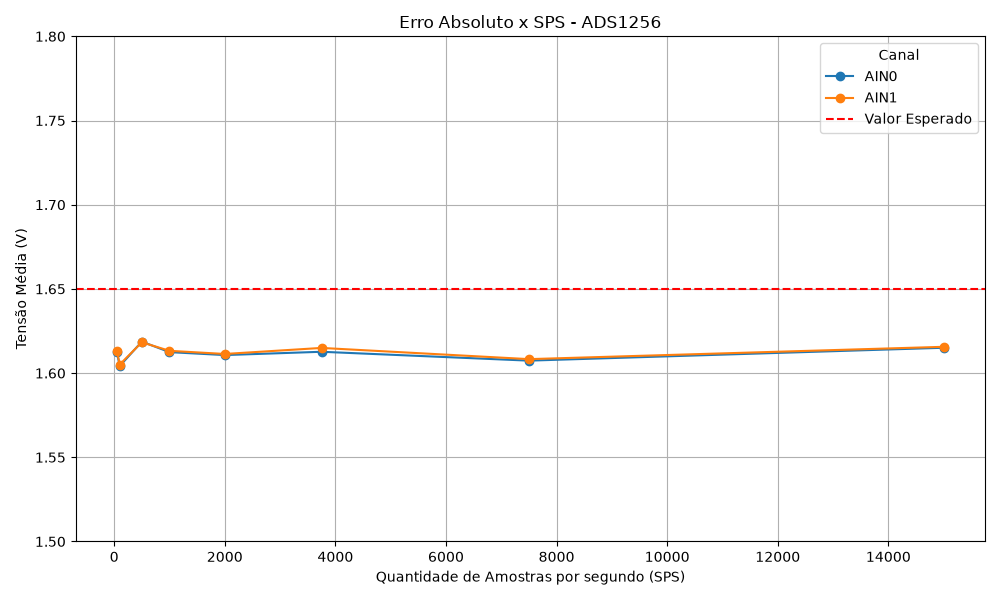
\includegraphics[width=0.9\textwidth]{grafico.png}}
    \caption{Tensão média medida em função da taxa de amostragem configurada no ADS1256.}
    \label{fig:grafico_sps}
\end{figure}

\section{Discussão}

Os resultados obtidos indicam que o ADS1256 apresentou desempenho adequado para a medição de uma tensão contínua conhecida em diferentes taxas de amostragem. 
Mesmo com o aumento do SPS, o erro absoluto permaneceu abaixo de 50 mV em todos os casos analisados. 
Isso sugere que o conversor é capaz de operar em taxas superiores às do ADC utilizado anteriormente, mantendo precisão suficiente para uma validação inicial do sistema.

Entretanto, não foi observada uma tendência clara de aumento do erro com o aumento do SPS. 
Em alguns casos, taxas de amostragem maiores apresentaram erros menores do que taxas menores. 
Esse comportamento não representa exatamente o esperado teoricamente, pois, em conversores delta-sigma, 
o aumento da taxa de amostragem tende a reduzir a filtragem digital efetiva, aumentando o ruído e reduzindo a resolução efetiva \cite{datasheet_ads1256}.

Essa diferença entre o comportamento esperado e os resultados obtidos pode estar relacionada às condições práticas do experimento. 
O teste foi realizado em protoboard, ambiente sujeito a ruídos elétricos, mau contato, resistência de contato e interferências externas. 
Além disso, a tolerância dos resistores, pequenas variações da alimentação de 3,3 V, ruído da fonte e diferenças entre o valor real do divisor e o valor esperado também podem influenciar os resultados.

Dessa forma, a aparente melhora da precisão em alguns valores maiores de SPS não deve ser interpretada como uma característica definitiva do ADS1256. 
O mais adequado é considerar que, dentro das condições experimentais utilizadas, o ADC conseguiu realizar medições próximas ao valor esperado para todos os valores de SPS testados. 

Ainda assim, o teste cumpre seu objetivo inicial: verificar se o ADS1256 é capaz de realizar medições válidas em diferentes taxas de amostragem. 
Considerando que todos os erros permaneceram abaixo do limite definido, 
os resultados indicam que o conversor é adequado para continuidade do desenvolvimento do sistema de coleta de dados.

\section{Considerações sobre o Uso dos 8 Canais}

Embora os testes realizados tenham utilizado apenas os canais AIN0 e AIN1, 
o projeto prevê o uso futuro de múltiplos sensores conectados ao ADS1256. 
Nesse contexto, é importante considerar o funcionamento do ADC ao utilizar todos os 8 canais.

O ADS1256 não possui um conversor independente para cada entrada analógica. 
Em vez disso, ele utiliza um multiplexador interno para selecionar qual canal será convertido em cada instante. 
Portanto, ao utilizar os 8 canais, as leituras não ocorrem simultaneamente, mas sim de maneira sequencial.

Esse comportamento tem impacto direto na taxa efetiva de amostragem por canal. 
Por exemplo, mesmo que o ADC seja configurado para 15000 SPS, ao alternar entre 8 canais a taxa efetiva estimada passa a ser de aproximadamente 477 SPS por canal, 
conforme apresentado na Tabela~\ref{tab:mux_8canais}. Assim, é importante não interpretar a taxa configurada como a taxa disponível em cada canal individualmente.

Esse aspecto é relevante para o sistema de coleta de dados, 
pois diferentes sensores podem exigir diferentes taxas de amostragem. 
Sinais lentos, como temperatura, podem ser coletados em taxas menores sem perda significativa de informação. 
Por outro lado, sinais mais dinâmicos, como aceleração, vibração ou empuxo durante eventos rápidos, podem exigir taxas de aquisição mais elevadas.

Portanto, para validar completamente o ADS1256 no sistema, não basta testar apenas um ou dois canais isolados. 
É recomendável realizar novos testes com todos os 8 canais conectados, preferencialmente com tensões conhecidas ou sinais de referência. 
Esse teste permitirá verificar a taxa efetiva por canal, a estabilidade das leituras, a influência da troca do multiplexador e a consistência entre os canais.

\section{Recomendações para Testes Futuros}

Para melhorar a confiabilidade dos resultados e validar o ADS1256 em condições mais próximas da aplicação real, recomenda-se realizar novos testes com as seguintes melhorias.

Primeiramente, é recomendável substituir a montagem em protoboard por uma placa de circuito mais estável, reduzindo ruídos, mau contato e interferências causadas pela montagem experimental.

Também é importante repetir cada teste mais de uma vez para cada valor de SPS. Com múltiplas repetições, 
será possível calcular média, desvio padrão e dispersão dos erros, obtendo uma análise estatística mais confiável.

Além disso, recomenda-se testar todos os 8 canais do ADS1256 conectados simultaneamente a valores conhecidos. 
Esse teste permitirá avaliar o comportamento do ADC ao alternar entre múltiplas entradas e verificar se a taxa efetiva por canal ainda atende às necessidades do sistema.

Outra melhoria importante seria utilizar uma fonte de tensão de referência mais estável, 
ou medir continuamente a tensão real do divisor com um instrumento de maior precisão. 
Isso ajudaria a separar o erro causado pelo ADC do erro causado pela própria tensão de entrada.

Por fim, recomenda-se realizar testes com sensores reais, como acelerômetros, células de carga e sensores de temperatura. 
Dessa forma, será possível avaliar não apenas a precisão em tensão contínua, mas também o desempenho do ADS1256 em sinais reais do sistema de coleta de dados.

\section{Conclusão}

Com base nos resultados obtidos, é possível afirmar que o ADS1256 apresentou precisão adequada para a medição de tensão no divisor resistivo em todos os valores de SPS testados. 
As leituras permaneceram próximas ao valor esperado de 1,65 V, com erro absoluto inferior ao limite de 50 mV adotado no teste.

Os canais AIN0 e AIN1 também apresentaram boa consistência entre si, com diferenças médias reduzidas. 
Isso indica que o ADS1256 foi capaz de realizar medições coerentes em ambos os canais avaliados.

Entretanto, os resultados não permitem concluir de forma definitiva a relação entre aumento do SPS e perda de precisão, 
pois não foi observada uma tendência clara de aumento do erro em taxas maiores. 
Esse comportamento pode ter sido influenciado pelas condições experimentais, especialmente pela montagem em protoboard e pela presença de ruídos externos.

De maneira geral, os resultados validam o uso inicial do ADS1256 no sistema de coleta de dados. 
O conversor demonstrou capacidade de realizar medições com erro aceitável em diferentes taxas de amostragem, 
representando uma melhoria em relação ao ADC de menor SPS utilizado anteriormente.

Como continuidade do projeto, recomenda-se realizar testes adicionais com todos os 8 canais conectados, 
montagem elétrica mais robusta, múltiplas repetições por taxa de amostragem e sensores reais. 
Esses testes permitirão caracterizar com maior precisão o desempenho do ADS1256 em condições próximas às da aplicação final.

\begin{thebibliography}{9}

\bibitem{datasheet_ads1256}
TEXAS INSTRUMENTS. \textit{ADS1255, ADS1256: Very Low Noise, 24-Bit Analog-to-Digital Converters}. Disponível em: \url{https://www.ti.com/lit/ds/symlink/ads1256.pdf}. Acesso em: 14 jun. 2026.

\bibitem{ti_e2e_fastcycling}
TEXAS INSTRUMENTS. \textit{ADS1256 fast cycling -- Data converters forum}. Disponível em: \url{https://e2e.ti.com/support/data-converters-group/data-converters/f/data-converters-forum/42575/ads1256-fast-cycling}. Acesso em: 14 jun. 2026.

\end{thebibliography}

\end{document}
